\textbf{Entrenadores y Atletas, que compartan el apellido y que se encuentren participando en la misma disciplina.
Deberan ordenar la información a partir del apellido paterno.}\vspace{.3cm}

Para esta consulta yo lo resolví de la siguiente manera: \vspace{.3cm}

\begin{lstlisting}
    SELECT 
        atleta.*,
        entrenador.identrenador,
        entrenador.nombre AS entrenador_nombre,
        entrenador.primerapellido AS entrenador_primerapellido,
        entrenador.segundoapellido AS entrenador_segundoapellido,
        entrenador.iddisciplina
    FROM 
        atleta
    JOIN 
        participa ON atleta.idatleta = participa.idatleta
    JOIN 
        entrenador ON entrenador.iddisciplina = participa.iddisciplina
    WHERE 
        (entrenador.primerapellido = atleta.primerapellido 
         OR entrenador.segundoapellido = atleta.segundoapellido)
    ORDER BY 
        atleta.primerapellido;
\end{lstlisting}

\textbf{Explicación:} \vspace{.3cm}

Lo que yo hice en esta consulta es, primero conseguir atletas y los iddisciplina de las disciplinas que practican, después, como los entrenadores para nosotros solo enseñan una disciplina, podemos tomar y unirlo por el iddisciplina, como no mencionan que apellido comparten o si el orden importaba, fui a lo sencillo, si el primer apellido del entrenador es igual al primer apellido del atleta o lo mismo para el segundo, entonces los seleccionamos, después ordenamos por el apellido paterno del atleta. \vspace{.3cm}

El resultado es una tabla con los datos de los atletas y para el entrenador nos da, su id, nombre, primer apellido, segundo apellido y la disciplina que enseña; todo ordenado por el apellido paterno del atleta. Una nota importante de esta consulta es que, como no se mencionan como deben aparecer los datos, si muchos atletas comparten algún apellido con 1 solo entrenador, nos regresara la información del entrenador muchas veces, y viceversa con los entrenadores (siempre y cuando cumplan con la condición de entrenar la misma disciplina). \vspace{.3cm}

\textbf{Resultado:}
\begin{center}
    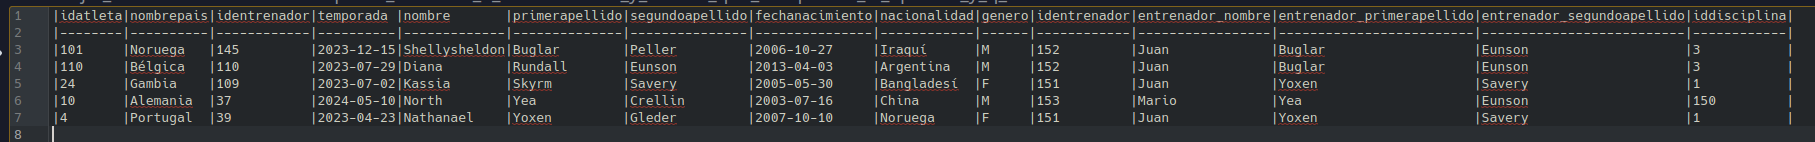
\includegraphics[width=1.05\textwidth]{resources/resultados/1.png}
\end{center}   

Otra aclaración importante es que lo que nos regreso fueron tuplas que yo añadi manualmente; agregue entrenadores con el mismo apellido que ciertos atletas e hice que coincidieran en la disciplina, para que se pudiera ver el resultado de la consulta. \vspace{.3cm}